%ब
\section{Solution3:  Metadata Column Family} \label{s:design-sol3}

In this approach,     metadata for all the column families in a keyspace is
stored in a separate column family called \texttt{Metadata}.   In this approach the metadata is
decoupled from the actual data and stored in a decentralised way where all the
\ac{PK} and \ac{FK} constraints of all the column families within a keyspace are
saved in a single location.  The other column families contain only the actual
data and does not store any metadata.  Using this approach,  all the constraints
as seen in Figure~\ref{fd:Metadata-Constraints} are saved as super columns in
the \texttt{Metadata} column family (Figure~\ref{fd:Metadata-Solution3}). 
 
	\begin{figure}[h] 
		\centering
		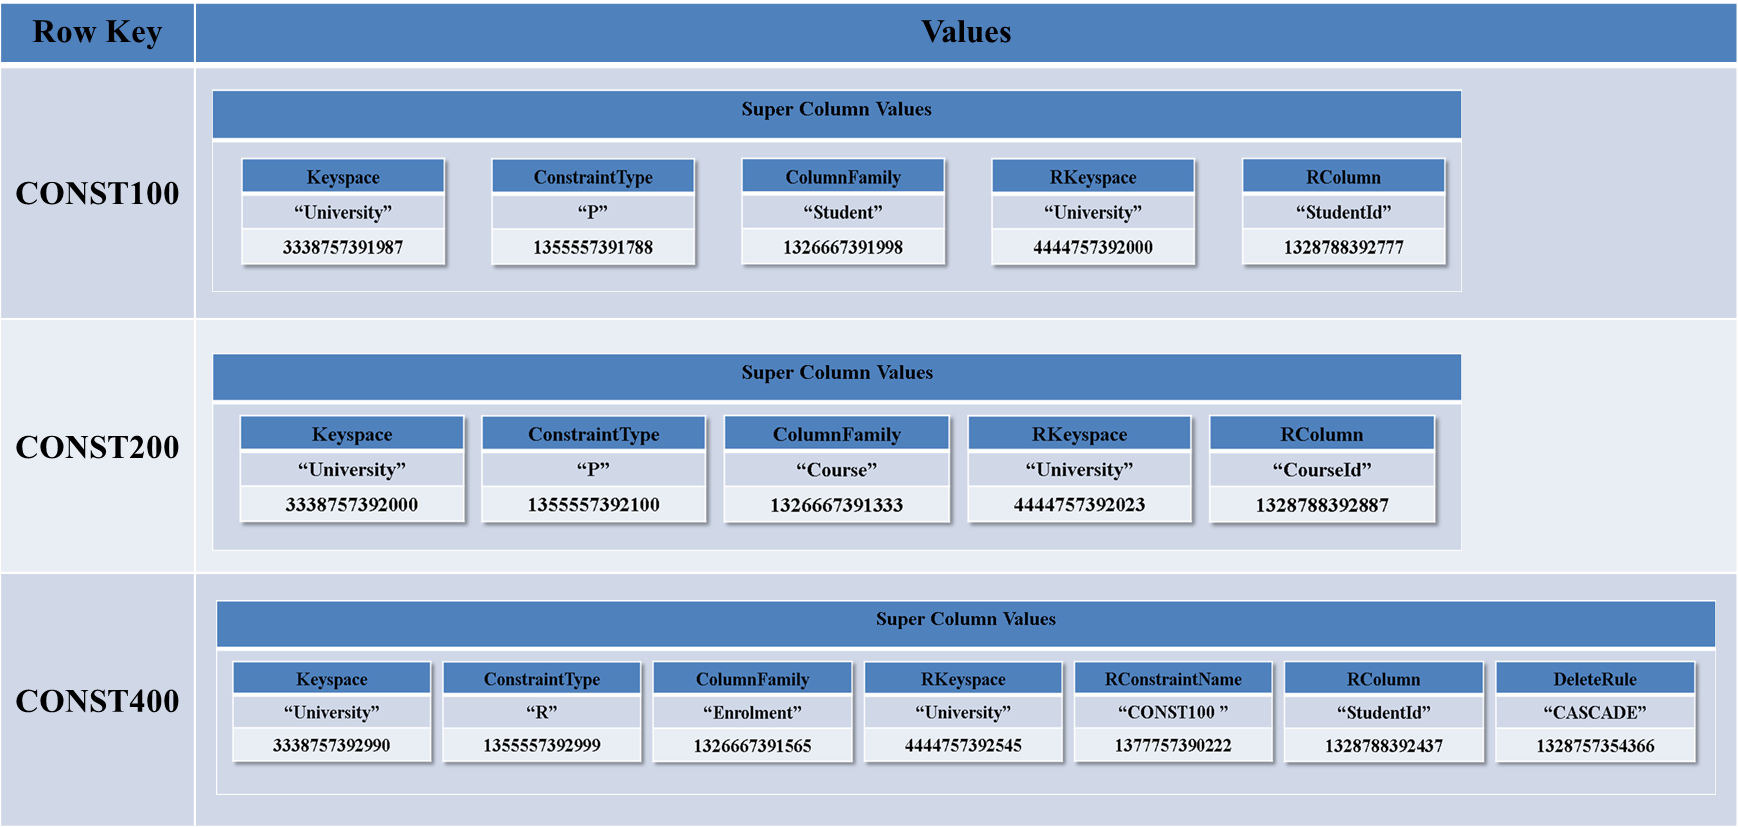
\includegraphics[width=.8\textwidth]{./figure/Solutions/Sol3-MD-ColumnFamily.png}
		\caption{Metadata Column Family in Solution 3}\label{fd:Metadata-Solution3}
	\end{figure}

The different parts of the constraints are saved as separate columns in the
\texttt{Metadata} column family. Thus,  no special characters are required to
identify the various parts as seen in Solutions~1 and 2.  When an operation is
invoked on a column family in the keyspace referential integrity validations
are triggered.  For these validations,  the experimental \ac{API} connects to
\texttt{Metadata} column family and retrieves the relevant constraints for the column family on
which the operation is invoked. 
The different parts of the constraints are accessed by identifying the
correct columns in the \texttt{Metadata} column family and necessary values are
retrieved to do the validation. 

This approach is similar to the way dependency information is
stored in traditional \acp{RDBMS},  where metadata holds information
about tables,  its dependencies and its many other properties.  Commonly,  such
metadata is maintained separately from the tables containing actual data and the
metadata is maintained in \texttt{System} tables.  
% Such tables  cannot be altered
% directly by the users and they can only query these tables for information. 
% Such an approach keeps metadata safe and away from users thus
% avoiding any mishandling of the metadata.  

The design to decouple metadata from the actual data is inspired from the
potential challenges in Solutions~1 and 2. 
% Such cases are when metadata undergoes frequent changes or a column family has
% many constraints. 
In Solutions~1 and 2,   a column family with several constraints will have a
large value in \texttt{Metadata} column and accessing as well as processing the
large metadata can consume more time.  Moreover,  in these solutions metadata has
to be changed at every place it is repeated in the event of any alterations to
the metadata. 
Consider Solution~1 where the \texttt{Metadata} column in every super column
of a column family has to be updated every time a constraint is added,  removed
or updated. 
In Solution~2,  the top row has to be changed for all the column families that have
any alterations  in their constraints.   

By decoupling metadata from the actual
data it is  easier to access and retrieve the various parts of the constraints
since these can be searched based on the column names once the constraint is
identified. 
More importantly,  it is now easier to add or remove constraints for a column
family since metadata  is centrally stored.  Any changes to metadata affects
only the \texttt{Metadata} column family and the experimental \ac{API} does not
have to access actual data to perform such changes. 
